\chapter{过时需求自动检测工具实现}

目前,针对过时需求自动检测问题,领域内还没有面向维护人员实际工具。在本章中,我们介绍了过时需求自动检测工具INFORM(IdeNtiFy Outdated RequireMents)的实现,INFORM集成了我们基于代码依赖关系的过时需求自动检测与更新推荐方法,并提供Console与GUI的版本。此外,INFORM的Console版本中集成了代码托管与版本控制服务GitHub的接口,使维护人员在向GitHub进行代码提交后,能够便利地获取潜在的过时需求,降低了需求更新参与一般维护过程的成本。

\section{系统体系结构}

图N展示了INFORM的系统体系结构,其中主要包括用户交互、代码版本比较,代码依赖静态分析,变更组构造及文本抽取,检索与推荐五大模块。在本小节中,我们将对上述五个模块的设计与实现进行说明。

\begin{figure}[thb]
    \centering
    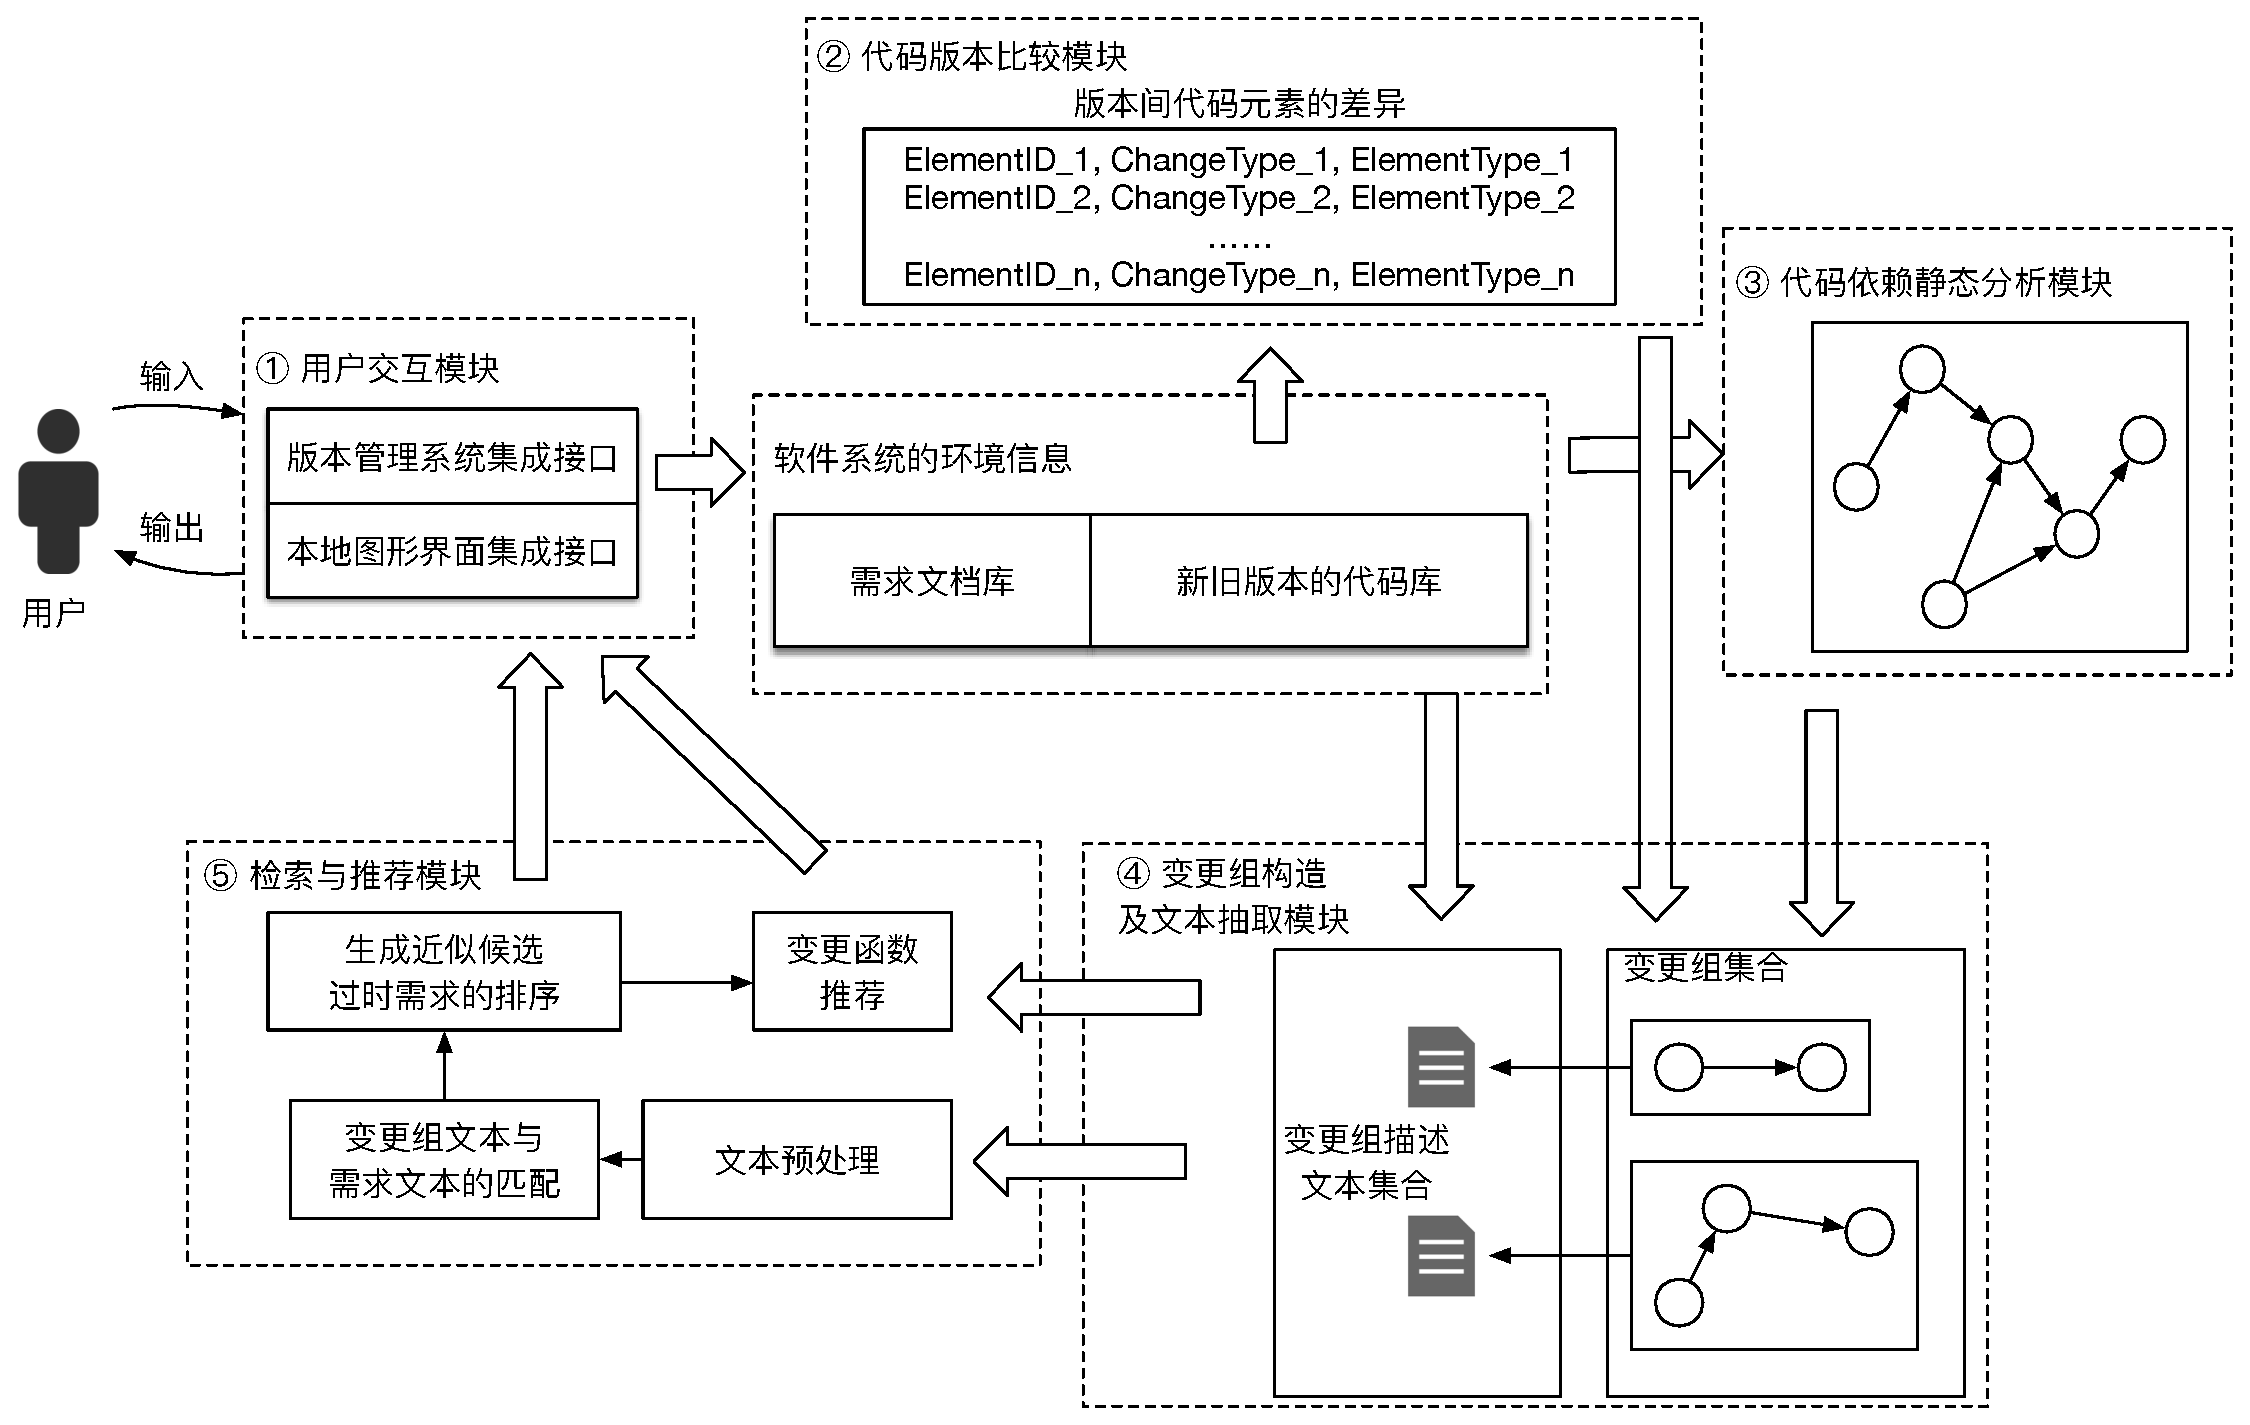
\includegraphics[width=1.0\textwidth]{./figures/inform/INFORM_Architecture.pdf}
    \caption{INFORM的系统体系结构图}
    \label{F:INFORM_Architecture}
\end{figure}

\begin{enumerate}
  \item 用户交互模块:INFORM通过此模块与用户(通常是维护人员)进行交互。用户较为熟悉的工具使用方式是图形界面或控制台,因此,INFORM的交互模块包含GUI与Console两个部分,它们共享同样的内核接口。

  以GUI版本的INFORM为例,对于任意一个软件项目,用户可以在文件系统中,指定需求,更新前后代码版本的路径,INFORM可以识别新旧版本间的代码元素差异并给予展示,用户此时可以通过点击界面的Retrieving按钮,以检测候选过时需求,检测结果将展示在当前界面的右上侧区域(如图N所示)。此外,用户可以选中其中的候选过时需求,并查看与该需求更新相关的变更函数的推荐,推荐结果展示在界面的左上侧区域。在GUI版本的INFORM的实现中,我们基于SWT(The Standard Widget Toolkit)完成了用户界面的设计,SWT提供了丰富的界面组件,能够满足INFORM的设计需要。

  对于Console版本的INFORM,我们将其与GitHub的接口相集成。用户只需提供项目的GitHub地址,需求的相对地址,并指定更新前后的代码版本号(CommitID),INFORM即可执行过时需求自动检测。
  \item 代码版本比较模块:在此模块中,INFORM比较了新旧两个版本代码间的差异,识别出其中的变更代码元素(包,类,函数,域)。在此过程中,我们基于Eclipse JDT(Java Development Tools)提取了源代码中的代码元素,并构造新旧版本的代码元素集合,通过比较集合间元素的不同,以识别出变更代码元素。

  \item 代码依赖静态分析模块:该模块主要负责代码依赖关系的抽取,其中包括函数的调用依赖及域的使用依赖。根据函数调用依赖的来源不同,对函数调用依赖的抽取有以下两种途径:(1)从编译后的字节码(Jar包)中抽取;(2)直接从代码的源文件(.Java为后缀的文件)中抽取。在前者的情况下,我们在静态分析时利用Apache BCEL库,析编译后的字节码以捕获代码的函数调用依赖。然而,在项目仓库中,对源码进行编译后产生的Jar文件通常是不可得的;在后者的情况下,经过我们的调研,没有发现能够直接从代码的源文件中抽取函数调用依赖的工具或类库。因此,我们基于Eclipse JDT对源码进行分析,实现了JDA(Java Dependencies Analyzer)工具,JDA可以直接分析代码的源文件并抽取函数调用依赖。域的使用依赖可以基于正则表达式的匹配获得。

  \item 变更组构造及文本抽取模块:首先,该模块基于获取的代码依赖关系,通过代码元素依赖的紧密度分析,可以获取与变更代码元素结构上紧密依赖的其他代码元素,以构成变更组。然后,模块根据变更组中代码元素的不同来源抽取关键词,从而构造变更组文本。通过词形还原,词根提取(Snowball Stemming)和去停用词等预处理技术标准化文本。

  \item 检索与推荐模块:
  在检索部分,该模块利用信息检索模型,计算变更组文本与需求文本的相似度矩阵,按照文本间相似度值发现近似候选过时需求。在此部分中,我们实现了词项-文档矩阵(TermByDocumentMatrix),相似度矩阵(SimilarityMatrix)等基础数据结构,以及VSM,JS与LSI这三个被广泛使用的信息检索模型。在推荐部分,结合代码依赖关系信息,模块基于TF-IDF的赋权技术,通过计算变更代码元素标识符中词汇的全局重要性和局部重要性以获取该变更代码元素的重要性,进行热点元素的推荐(详见x.x.x节)。
\end{enumerate}

\section{案例分析}

\section{运行时系统行为}

\section{本章小结}